\section{Modeling and Simulation}
\label{sec:modeling_and_simulation}
For the purpose of doing design verification and optimization, a simplified model of the robot was created. The model was created in Simscape, a physical modeling toolbox integrated with MATLAB/Simulink. 

\subsection{Simscape}

Simscape is a simulation tool that allows you to rapidly create models of physical systems within Mathworks' MATLAB/Simulink environment. With Simscape, physical systems are built by interconnecting blocks representing physical components, such as rigid bodies, joints and springs in a block diagram. The blocks are parameterized by physical properties, such as mass, inertia, and damping. Simscape automatically generates the equations of motion for the system, which can be solved numerically to simulate the system's behavior. Like you can do with Simulink without Simscape, you can also add ordinary Simulink blocks, including Matlab Function blocks, to the model. Simscape is also compatible with Simulink's multiple numerical solvers, such as ode15s, ode45, and ode23s (TODO? Is it ode23t?). 

An example of a typical SimScape block diagram can be found in figure \ref{fig:simscape_tutorial_diagram}. A visualization of the corresponding model can be seen in figure \ref{fig:simscape_tutorial_visualization}. As one can see, each element in a block diagram is typically either a rigid body, or joints connecting the various rigid bodies. Since a given body has multiple possible locations that a joint could be connected to, as well as axes it can act on, blocks can export different frames, with different origins and orientations, depending on the desired position and orientation of the joint. For example, for a block representing the robotic equivalent of a thigh, natural output frames would be the ones with origins at the top and bottom of the thigh, with a select axis aligned with the desired knee or hip axis of rotation. TODO: We want to use something other than the tutorial here, but our robot model is too split into submodels of submodels, so it loses the intuition you get from a "flatter" model. Will fix later. 

\begin{figure}
    \centering
    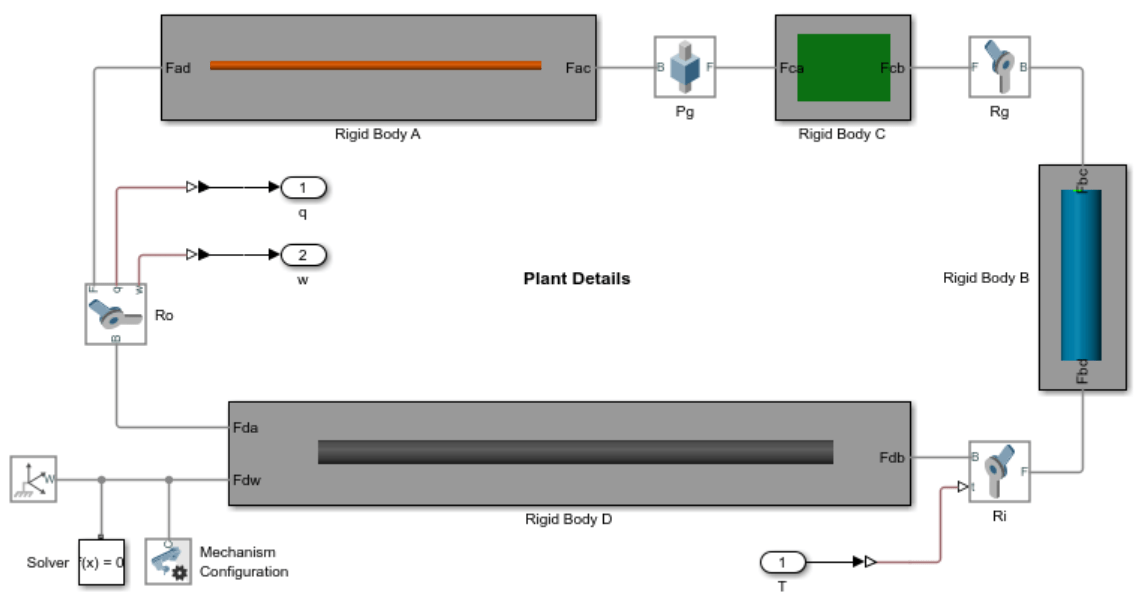
\includegraphics[width=0.5\textwidth]{Images/simscape_tutorial_diagram.png}
    \caption{A typical Simscape block diagram.}
    \label{fig:simscape_tutorial_diagram}
\end{figure}
\begin{figure}
    \centering
    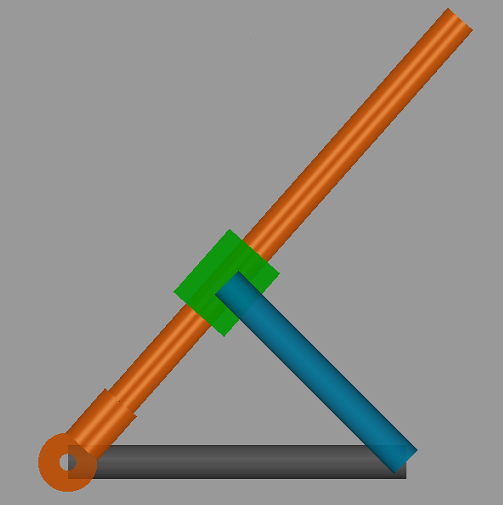
\includegraphics[width=0.5\textwidth]{Images/simscape_tutorial_visualization.png}
    \caption{A visualization of the model in figure \ref{fig:simscape_tutorial_diagram}.}
    \label{fig:simscape_tutorial_visualization}
\end{figure}

\subsection{Rigid Body Components of the Robot Model}
\label{sec:robot_main_parts}

Since the purpose of the Simscape model is not to facilitate the development of a complicated full degree of freedom feedback controller, nor to optimize every small detail of the design, a simplified model was selected. This model consists of a main body with four legs, each of which with two degrees of freedom. A visualization of the model, as well as an overview of the body's naming conventions can be found in figure \ref{fig:name_conventions}. An overview of the body's angle conventions can be found in figure \ref{fig:angle_conventions}. Note the absence of a hip abduction/adduction joint. This is because the model's main purpose is to verify the design for jumping in the sagittal (forward-backward and upwards-downwards) plane, and the hip abduction/adduction joint is not necessary for this purpose.

Regarding the naming conventions presented in figure \ref{fig:name_conventions}, note especially the naming of the different legs corresponding to location on the body, namely RH (Right Hind), RF (Right Front), LH (Left Hind), and LF (Left Front). Note also the naming of the joints hip (HIP) and knee (KNEE). If you see the angle conventions in figure \ref{fig:angle_conventions}, you can see that the angles of these joints correspond to the angles $\theta_1$ and $\theta_2$ respectively. Note that an orientation of zero degrees for the hip joint corresponds to the leg pointing straight downwards, and an orientation of zero degrees for the knee joint corresponds to the shank pointing in the same direction as the thigh. 

TODO: Add body coordsys in both figures? So I can explain that positive rotation for both sides corresponds to positive rotation about the body y axis in nominal position. 

As can be seen in both figure \ref{fig:name_conventions} and figure \ref{fig:angle_conventions}, in addition to the main body and legs colored in grey, the robot model also contains large purple blocks. These blocks represent motor masses, and their mass can be adjusted to represent different motors. 

\begin{figure}
    \centering
    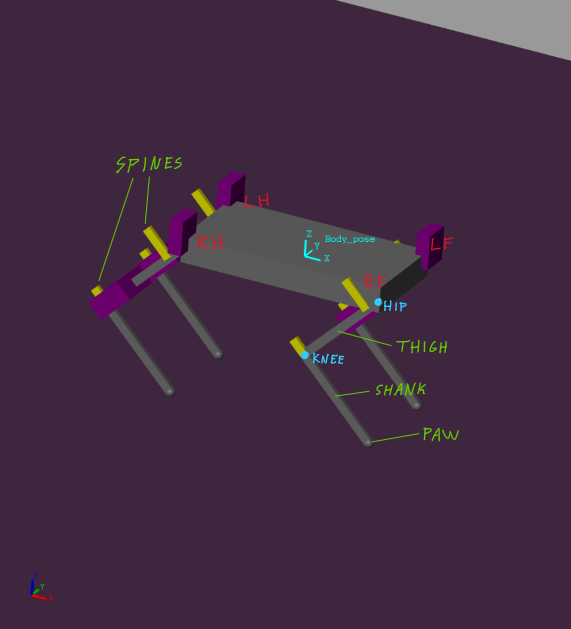
\includegraphics[width=0.5\textwidth]{Images/name_conventions.png}
    \caption{Naming conventions for the parts of the robot, as well as forwards direction definition. TODO: name spines}
    \label{fig:name_conventions}
\end{figure}

\begin{figure}
    \centering
    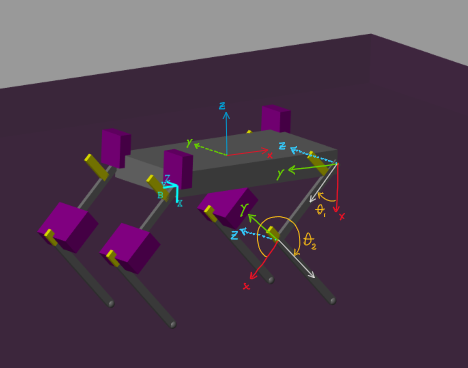
\includegraphics[width=0.5\textwidth]{Images/angle_conventions.png}
    \caption{Angle conventions for the robot body.}
    \label{fig:angle_conventions}
\end{figure}

\subsection{Rigid Body Masses and Inertias}
\label{sec:mass_inertia_properties}

In Simscape, the mass and inertia properties of a rigid body can be specified by the user or automatically calculated based on the body's geometry and material properties. Hybrid solutions are also possible, where the user specifies some properties and Simscape calculates the rest \cite{simscape_tutorial}. 

In the case of this model, a summary of the origin of the mass and inertia properties of the rigid bodies can be found in table \ref{tab:mass_inertia_properties}. Exceptions are the properties of the main body and the paws, which will be specified in more detail in the two next paragraphs. For the parts whose mass and inertia are calculated by the geometry, this geometry will be specified in detail whenever the model is used, for example, section ref: TODO, the link-length optimization section, will specify the geometry assumed during the optimization. 

The mass properties of the main body are based on the hardware components used by the Eurepus robot constructed by Maurer and El Agroudi \cite{finn_tarek_master}. Since early in the design process a rough estimate was needed for the robot body mass, and it seemed likely that the electronic solution, apart from the motors, would be similar to the Eurepus robot, an approximate mass of the main body was calculated based on the mass of some of the Eurepus robot's electronics plus an approximate amount of Nylon body material, four motors, and a random chosen microcontroller (MCU) mass. The formula used for the approximate of the main body mass can be found in equations \ref{eq:Nylon_plate} to \ref{eq:main_body_mass}. The masses corresponding to variables in equations \ref{eq:Nylon_plate} to \ref{eq:main_body_mass} can be found in table \ref{tab:component_masses}. The motor mass chosen in table \ref{tab:component_masses} corresponds to the mass of the agfrc A20BHM motor, this motor was chosen because it is unlikely that the hip abduction/adduction motor will be any heavier than this, for details, see section \ref{sec:robot_design} or robot hardware? TODO. 

The geometrical, mass and inertia properties of the paws differ based on which of two scenarios we intend to simulate. The first scenario is the normal jumping scenario, in which the paw mass is simply set to 1000 $kg/{m^3}$, though choosing the actual density of rubber would maybe be more appropriate. The dimensions of the paw are in this scenario simply chosen so that the diameter coincides exactly with $max(\text{shank width, shank height})$. The second scenario was meant to test the leg motor's potential ability to do in air attitude stabilization like done in \cite{finn_tarek_master}. This scenario will be described in more detail in section TODO. 

\begin{table}
\centering
\begin{tabular}{|c|c|c|c|c|}
\hline
\textbf{Component} & \textbf{Mass} & \textbf{Density (kg/m$^3$)} & \textbf{Inertia} & \textbf{Geometry} \\
\hline
Main Body & See section \ref{sec:mass_inertia_properties} & See section \ref{sec:mass_inertia_properties} & See section \ref{sec:mass_inertia_properties} & Rectangular Prism \\
Thigh & From geometry & 2700 (Aluminium 6061) & From geometry & Rectangular Prism \\
Shank & From Geometry & 2700 (Aluminium 6061) & From Geometry & Rectangular Prism \\
Law & From Geometry & 2700 (Aluminium 6061) & From Geometry & Rectangular Prism \\
Hip Motor & Actual motor mass & From Geometry & From Geometry & Rectangular Prism \\
Knee Motor & Actual motor mass & From Geometry & From Geometry & Rectangular Prism \\
Thigh Spine & From Geometry & 2700 (Aluminium 6061) & From Geometry & Rectangular Prism \\
Shank Spine & From Geometry & 2700 (Aluminium 6061) & From Geometry & Rectangular Prism \\
Paw & See section \ref{sec:mass_inertia_properties} & See section \ref{sec:mass_inertia_properties} & See section \ref{sec:mass_inertia_properties} & Sphere \\
\hline
\end{tabular}
\caption{Mass and inertia properties of the rigid bodies in the robot model. A list of the Eurepus robot's electronics can be found in \cite{finn_tarek_master}. }
\label{tab:mass_inertia_properties}
\end{table}

\begin{equation}
\label{eq:Nylon_plate}
m_{plate} = \rho_{nylon} \cdot V_{plate} = \rho_{nylon} \cdot l_{plate} \cdot w_{plate} \cdot h_{plate}
\end{equation}

\begin{equation}
\label{eq:eurepus_electronics}
m_{\text{eurepus\_electronics}} = m_{\text{battery}} + m_{\text{I2C}} + 12 \cdot m_{\text{ADC}} + m_{\text{PWM\_driver}}
\end{equation}

\begin{equation}
\label{eq:main_body_mass}
m_{\text{main\_body}} = m_{\text{plate}} + m_{\text{eurepus\_electronics}}+m_{MCU}+ 4 \cdot m_{\text{motor}}
\end{equation}

\begin{table}
\centering
\begin{tabular}{|c|c|c|}
\hline
\textbf{Variable} & \textbf{Description} & \textbf{Value} \\
\hline
$\rho_{nylon}$ & Density of Nylon & 1520 kg/m$^3$  \\
$l_{plate}$ & Length of the plate & 10 cm \\
$w_{plate}$ & Width of the plate & 6 cm \\
$h_{plate}$ & Height of the plate & 1.67 cm \\
$m_{\text{battery}}$ & Mass of the battery & 27 g  \\
$m_{\text{motor}}$ & Mass of one motor & 20 g  \\
$m_{\text{I2C}}$ & Mass of the I2C module & 5.1 g  \\
$m_{\text{ADC}}$ & Mass of one ADC module & 2.4 g  \\
$m_{\text{PWM\_driver}}$ & Mass of the PWM driver & 8.5 g  \\
$m_{MCU}$ & Approximate mass of some microcontroller & 30 g \\
$m_{\text{main\_body}}$ & Resultant mass of the main body & 332 g \\
\hline
\end{tabular}
\caption{Masses and dimensions used in the main body mass calculation.}
\label{tab:component_masses}
\end{table}


\subsection{Elastic Components: Springs}

In addition to the model's many rigid bodies, we also implemented two different forms of spring based passive actuation, namely: 
\begin{itemize}
\item \textbf{A torsional spring} acting in parallel with the knee joint, as illustrated in figure TODO. This spring is at zero extension when the knee joint is at zero degrees, and applies a torque that is proportional to the knee joint angle, as covered in section \ref{sec:spring_theory}.
\item \textbf{An extension spring} acting in parallel with the knee joint, attached to the shank and thigh spine, as illustrated in TODO: add figure illustrating spines/add spine description in main body figure. The force generated by the extension spring is proportional to the displacement of the shank from the thigh, as covered in section \ref{sec:spring_theory}.
\end{itemize}

The torsion spring was implemented in the model using Simscape's prismatic joint option to add spring stiffness. The extension spring, on the other hand, was connected in parallel to the joint using Simscape's natural block diagram functionality, as seen in figure \ref{fig:simscape_extension_spring}. 

\begin{figure}
    \centering
    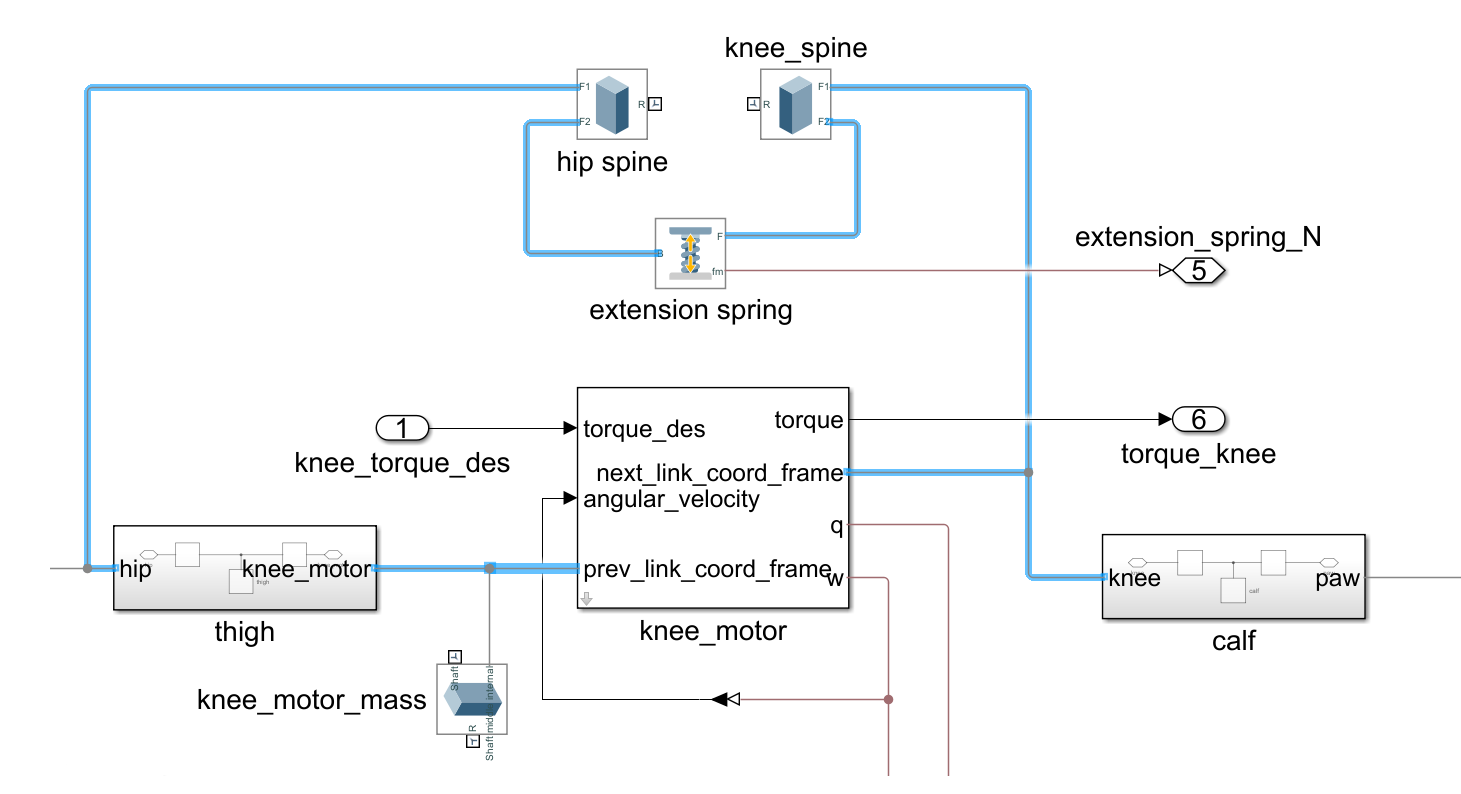
\includegraphics[width=0.5\textwidth]{Images/simscape_extension_spring.png}
    \caption{Extension spring implementation in Simscape. As can be seen, the spring is connected between the appropriate points (output frames) of the thigh and shank spine, and in parallel to the knee motor model, which contains the knee joint.}
    \label{fig:simscape_extension_spring}
\end{figure}

\subsection{Motor Modeling}
\label{sec:motor_modeling}

To be able to more accurately judge the jumping capability of different motors, a motor model in the form of a torque speed curve was implemented. The BLDC torque-speed curve presented in figure \ref{fig:bldc_torque_speed} is characterized by four parameters, namely the stall torque, the operating torque, the rated speed, and the maximum speed. Since motor suppliers contacted (primarily agf-rc and T-motor) were unable to provide most of the desired parameters, we chose a motor model with only two parameters, namely stall torque and maximum speed. The torque-speed model thus became a simple model where torque decreases linearly from stall torque, at speeds smaller than or equal to zero, to zero at speeds greater than or equal to maximum speed. The model is identical for negative velocities and torques, but with opposite signs. An example of the relation between desired torques and achieved torques for a given motor max speed can be seen in figure \ref{fig:torque_speed_func}.

\begin{figure}
    \centering
    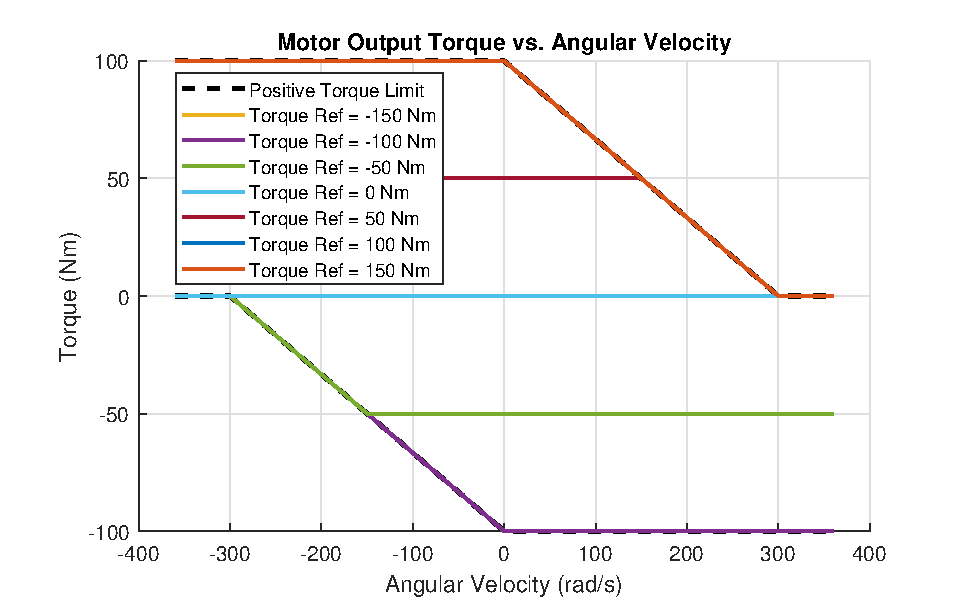
\includegraphics[width=0.5\textwidth]{Images/torque_speed_func.eps}
    \caption{Torque-speed characteristics of the motor.}
    \label{fig:torque_speed_func}
\end{figure}

\subsection{Solver selection}

As described in section \ref{sec:spring_theory}, the potential energy of a loaded spring can be easily calculated. Similarly, the potential energy due to gravity of a robot at the peak of a jump can also be determined. For the reasons discussed in section \ref{sec:numerical_solvers} we chose a stiff numerical solver, initially, we chose the ode15s solver. However, it was eventually observed that simulations using ode15s occasionally resulted in jump trajectories where the gravitational potential energy at the robot's peak height exceeded the combined potential energy of the four fully loaded springs by a factor of 2, even for jumps with only passive (spring) actuation. To address this inaccuracy, we experimented with different numerical solvers and ultimately selected the ode23s solver. This solver provided accurate simulations without artificially generating excess energy, and it performed efficiently.

%\subsection{Simscape}
%Simscape is a physical modeling toolbox integrated with MATLAB/Simulink. While Simulink handles signal-based modeling through block diagrams, Simscape adds the ability to model physical components and their interactions directly. For this project, its multibody library was used to create a simplified model of the robot. The key advantage is automatic handling of complex multi-body dynamics equations. Rather than manual derivation, Simscape generates them based on specified geometry and joints. The model parameters can be easily modified through MATLAB scripts.

%\subsection{Motor Torque-Speed Characteristics}
%To model the motor torque-speed characteristics, a torque-speed curve such as the one covered in section \ref{sec:theory:motor_model} was used, with parameters as covered in section \ref{sec:hardware:motor_characteristics}.



%\subsection{Motor Friction Modelling}
%Since the motors will be turned off during the jumping maneuver, motor friction must be included. It was modelled using a linear motor friction model covered in section \ref{sec:theory:motor_model}, using only the viscous friction component. To estimate the model parameters, we performed hardware tests for each motor, where the motors acted as the axis of rotation for a pendulum. A aluminium rod with a aluminium ballast was attacted to the motor shaft, and the pendulum was released from rest at horizontal position and allowed to swing freely untill at rest. This was repeated for both motors. The tests where filmed by a phone camera placed at a distance in front of the pendulum, and the angles of the pendulum were manually annotated using Tracker \cite{tracker}. The hardware setup is shown in figure \ref{fig:motor_friction_test_setup}, and the results are shown in figure \ref{fig:results:motor_friction_test}.

